\documentclass[12pt,a4paper]{report}

%Set language
\usepackage[english]{babel}
\usepackage{enumerate}

% To import and adjust images
\usepackage{graphicx}
\usepackage[export]{adjustbox}
\usepackage[center]{caption}
\usepackage{subcaption}
\usepackage{float}
\usepackage{tabularx}

% To use monospaced font
\usepackage{courier}

% To build a clickable Toc
\usepackage{color} %May be necessary if you want to color links
\usepackage{hyperref}
\hypersetup{
    colorlinks=true, %set true if you want colored links
    linktoc=all,     %set to all if you want both sections and subsections linked
    linkcolor=black,  %choose some color if you want links to stand out
    urlcolor = black
}


%To load PoLitecnico's logo
\usepackage{titling}

% Command to hide subsections in the Toc
\setcounter{tocdepth}{1}

% I don't like dots in the Toc
\usepackage{tocloft}
\renewcommand{\cftdot}{}

%To improve the tables
\usepackage[table]{xcolor}

%To break line inside tables
%\usepackage[utf8]{inputenc}
%\usepackage{fourier} 
%\usepackage{array}
\usepackage{makecell}
%\renewcommand\theadalign{bc}
%\renewcommand\theadfont{\bfseries}
\renewcommand\theadgape{\Gape[4pt]}

% Path relative to the .tex file containing the \includegraphics command
\graphicspath{ {./images/} }

% To change the ToC title
\addto\captionsenglish{ \renewcommand {\contentsname} {Table of
contents}}

%logo
\pretitle{
	 \begin{center}
	 \LARGE
	 
\includegraphics[width = 0.6\textwidth]{logo}\\[\bigskipamount]
}
\posttitle{\end{center}}

% Here we go
\title{Artificial Neural Networks and Deep Learning \\ Homework 1 - Image Classification}
\author{Frantuma Elia - 10567359 - 945729, \\
		Fucci Tiziano - 10524029 - 946638}
\date{A.Y. 2020/2021}

\begin{document}
	\maketitle
	%Index
	\tableofcontents
	\chapter{Introduction}
		\section{Description of the task}
			The homework consists in an image classification problem on the proposed dataset. In particular, it is required to classify images depicting groups of people based on the number of masked people. In the specific, the solution must discriminate between images depending on the following cases:

\begin{enumerate} 
	\item no person in the image is wearing a mask;
	\item all the people in the image are wearing a mask;
	\item someone in the image is not wearing a mask.
\end{enumerate}
In the following figure, one sample image for each class is shown.

\begin{figure}[H]
\renewcommand*\thesubfigure{\arabic{subfigure}} 
\centering
\begin{subfigure}{.3\textwidth}
  \centering
  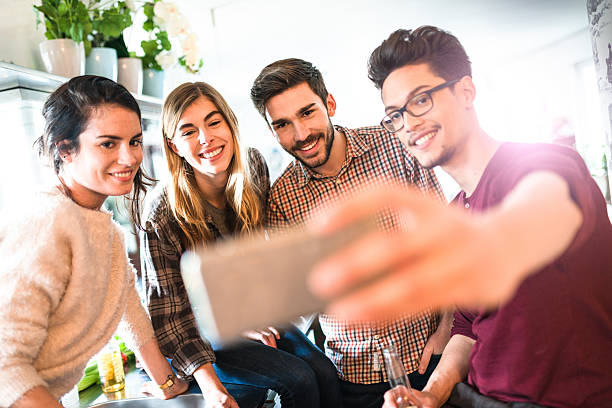
\includegraphics[width=1\linewidth]{image0}
  \caption{}
  \label{fig:sub1}
\end{subfigure}
\begin{subfigure}{.3\textwidth}
  \centering
  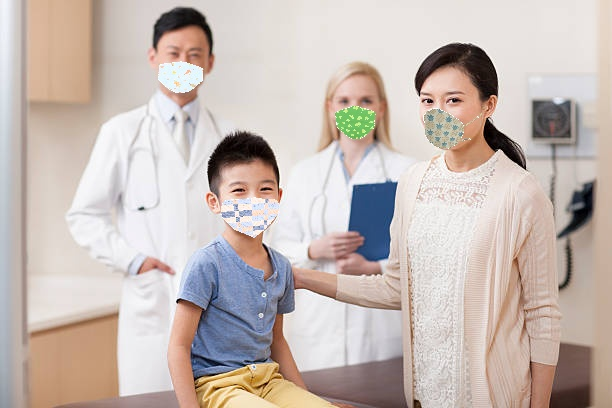
\includegraphics[width=1\linewidth]{image1}
  \caption{}
  \label{fig:sub2}
\end{subfigure}
\begin{subfigure}{.3\textwidth}
  \centering
  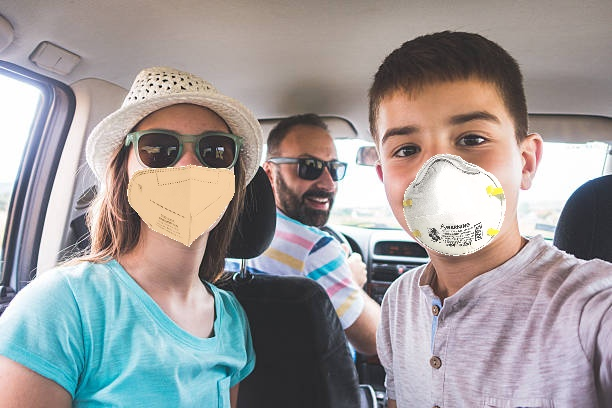
\includegraphics[width=1\linewidth]{image2}
  \caption{}
  \label{fig:sub3}
\end{subfigure}
\end{figure}

Thus, the classification is performed on 3 different classes. Being a classification problem, given an image, the goal is to predict the correct class label.

	\section{Dataset}

The dataset is composed by .jpg images of different size, divided in two folders:
			\begin{itemize}
				\item training (5614 images)
				\item test (450 images)
			\end{itemize}

A JSON file, containing the labels of the training images, is attached to the dataset.
The dataset requires the training images to be divided into three folders (created manually), corresponding to the three target classes. The division was done with a python script, which is contained in the notebooks.

\textit{Note: the dataset path expected by the script is:}

 ..\textbackslash\textbackslash artificial-neural-networks-and-deep-learning-2020\textbackslash\textbackslash MaskDataset

	\subsection{Data augmentation}
We have performed data augmentation in order to increase the dataset dimension. Some of the parameters used to perform the transformations are: brightness, zoom, horizontal/vertical shift and flip.
We didn't use rotation, since we noticed that the filling could reduce the performance of the classifier.

	\section{Validation set}

No automatic validation set is provided. This means that a subset of the training set must be used to perform validation.

In our case, we parametrized the number of training images to be moved into the validation set, with values between 3-15\%.


	\section{Test set}
The test set was left untouched, apart from the creation of one directory, named ``unlabeled'', which contains all the images.
	\section{Evaluation}
Submissions are evaluated on multiclass accuracy, which is simply the average number of observations with the correct label.
To submit a prediction, it is necessary to produce a .csv file containing the predictions associated to each test image. This file has to be submitted to the Kaggle page of the competition to obtain the accuracy score on the test set.

	%end of first chapter

	\chapter{Neural network architecture}
		\section{Ex-novo architecture}
	First, we tried to build a sequential neural network from scratch: we made many experiments, each one with a slightly different parameter configuration. Among them:
			\begin{itemize}
				\item \texttt{start\_f}: the number of initial filters;
				\item \texttt{depth}: the number of convolutional layers;
				\item the learning rate;
				\item the batch size;
				\item the size of the input image;
				\item the shape of the neuron activation function;	
				\item the number of fully connected layers.
			\end{itemize}
	After few experiments, we found that the best model was a convolutional neural network having \texttt{start\_f = 9} and \texttt{depth = 7}. The complete model of the network is descripted in the attached file \texttt{HomeworkImages.ipynb}.
		\subsection{Score}
	The best score of the network was 0.85555, obtained with the following settings:
	\begin{itemize}
		\item	\texttt{start\_f = 9};
		\item	\texttt{depth = 7};
		\item image resolution: 348x522;
		\item batch size = 8;
		\item two fully connected layers, made of 512 and 256 neurons.
	\end{itemize}
		\subsection{Diagrams}
Here we show how loss and accuracy changed during the network training, both for the training (grey) and the validation set (orange).
		\begin{figure}[H]
			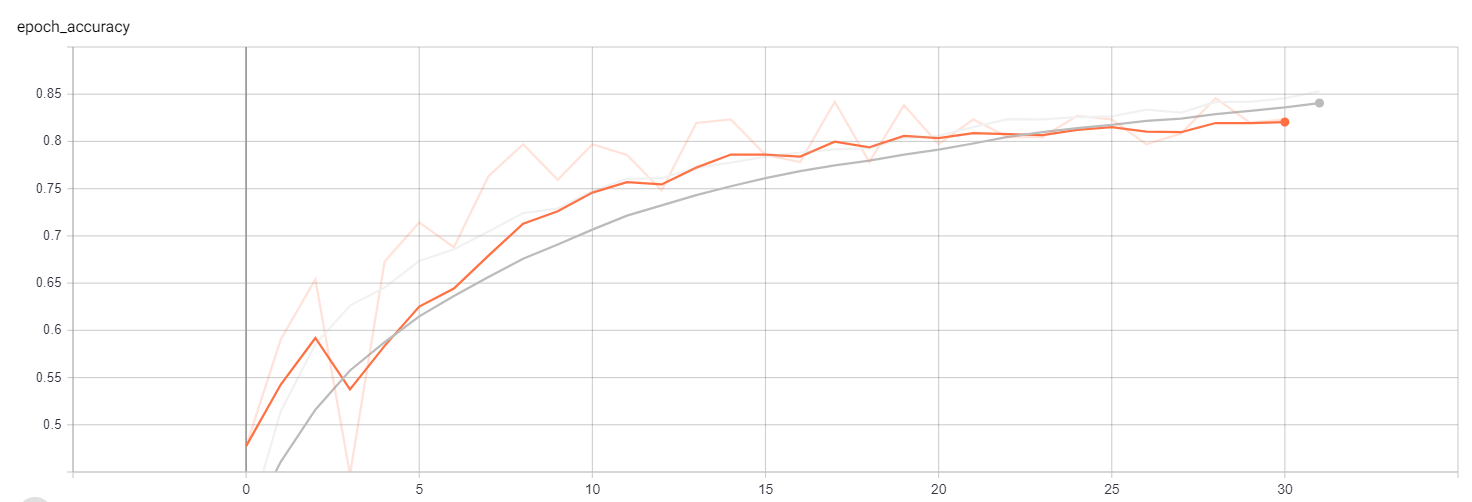
\includegraphics[scale = 0.5, center]{ex-Novo accuracy}
			\caption{Accuracy plot}
		\end{figure}
		\begin{figure}[H]
		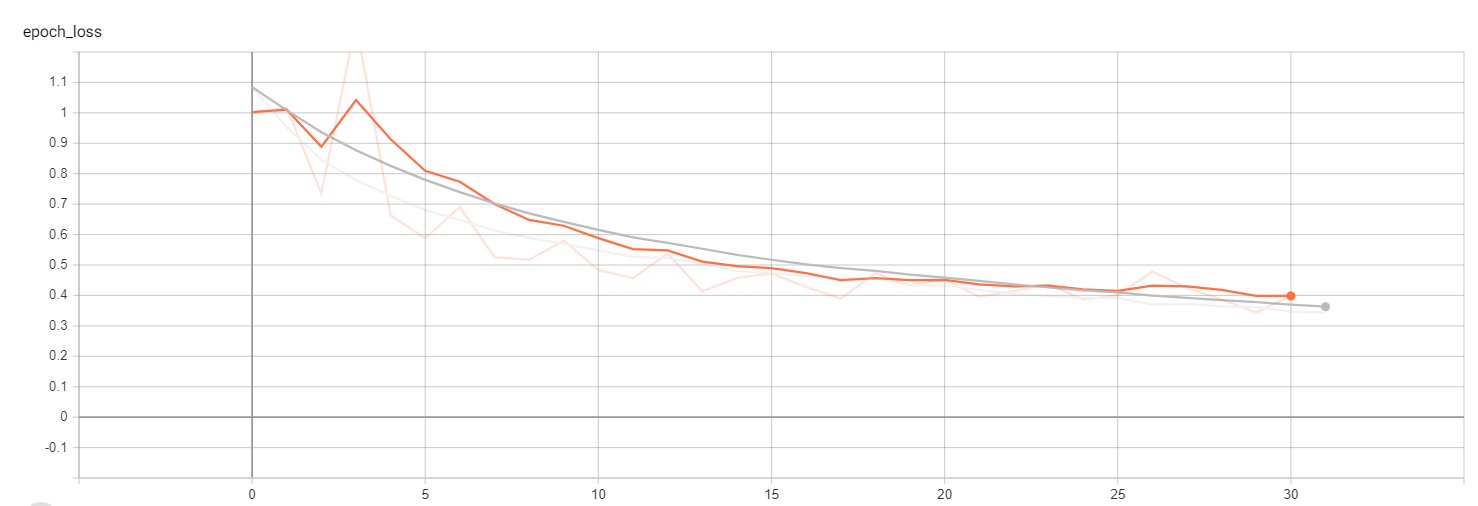
\includegraphics[scale = 0.5, center]{ex-Novo loss}
		\caption{Loss plot}
		\end{figure}
		
		\section{Transfer learning with VGG}
	The final version of the ex-novo architecture was pretty accurate, but we could not achieve better results by just changing the parameters. We decided to use a pre-trained, reliable and successful architecture.\\
	Our first try was with VGG16, because we've seen it during the lectures. Also in this case we made many experiments, each one with a different parameter configuration:
	\begin{itemize}
		\item \texttt{freeze\_until}: the layer of the network from which we want to fine-tune;
		\item the learning rate;
		\item the size of the input image;
		\item the shape of the neuron activation function;	
		\item the number of fully connected layers.
		\item the number of neurons in fully connected layers.
	\end{itemize}
		\subsection{Score}
The best score of the network was 0.89333, obtained with the following settings: 
	\begin{itemize}
		\item	\texttt{freeze\_until = 11};
		\item one fully connnected layer with 32 neurons before the softmax layer.
	\end{itemize}

		\subsection{Diagrams}
Here we show how loss and accuracy changed during the network training, both for the training (grey) and the validation set (orange).
		\begin{figure}[H]
			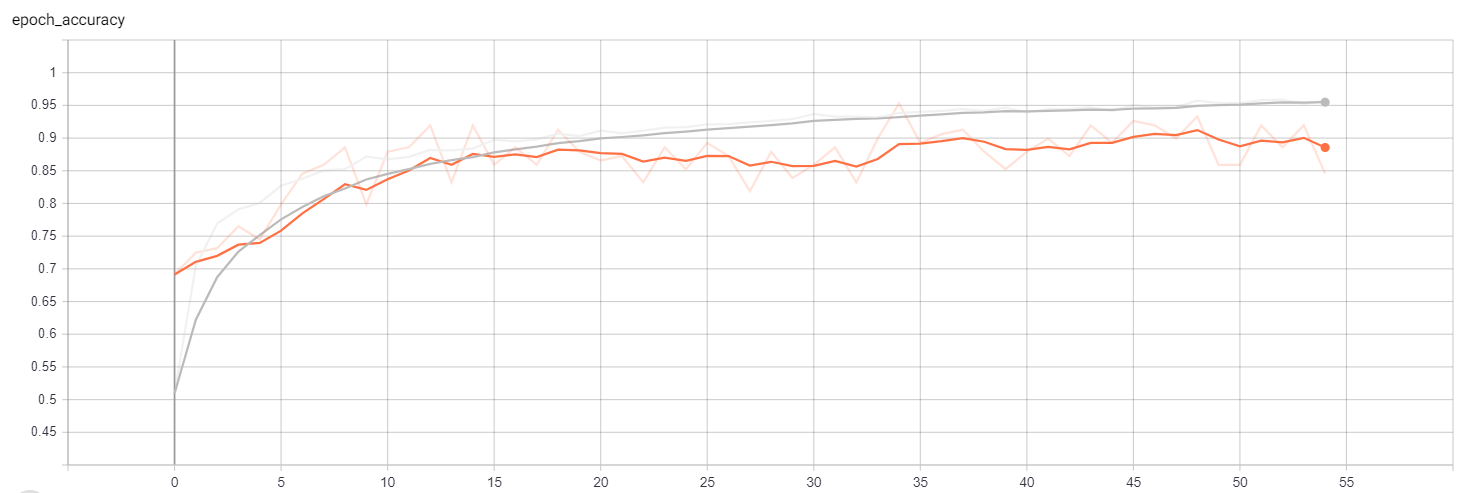
\includegraphics[scale = 0.5, center]{vgg accuracy}
			\caption{Accuracy plot}
		\end{figure}
		\begin{figure}[H]
			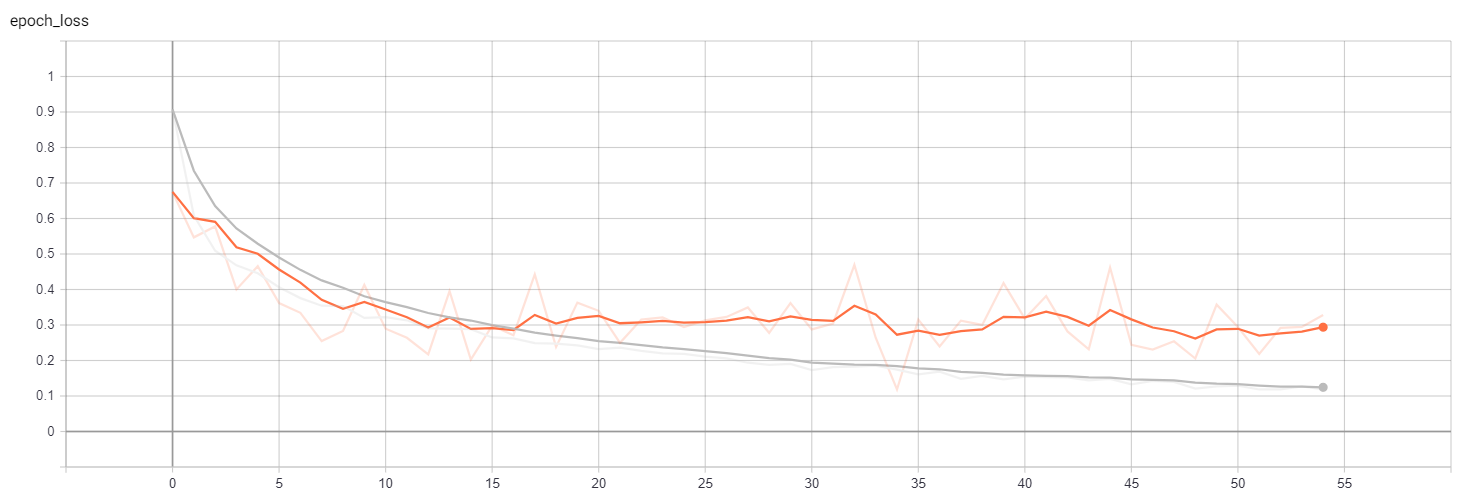
\includegraphics[scale = 0.5, center]{vgg loss}
			\caption{Loss plot}
		\end{figure}

\section{Transfer learning with ImageResNetV2}
For our last attempt we decided to use ImageResNetV2, the best performing on the ImageNet dataset. The approach in this case has been similar to the one with VGG, since we only changed the backbone. One significant change that has been made is the replacement of the fully connected layer(s) with a Global Average Pooling layer.
\subsection{Score}
	The best score of the network was 0.96888, obtained with the following settings:
	\begin{itemize}
		\item	\texttt{freeze\_until = 150};
		\item image resolution: 348x522;
		\item batch size = 8.
	\end{itemize}
\subsection{Plots}
Here we show how loss and accuracy changed during the network training, both for the training (grey) and the validation set (orange).
\begin{figure}[H]
	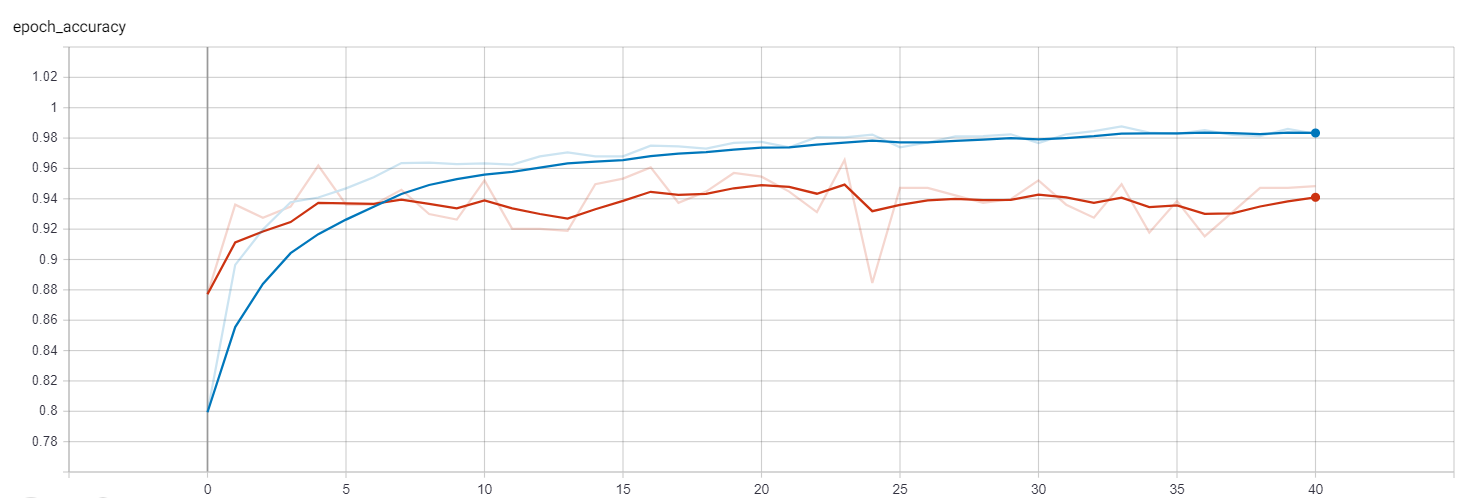
\includegraphics[scale = 0.5, center]{ResNet accuracy}
	\caption{Accuracy plot}
\end{figure}
\begin{figure}[H]
	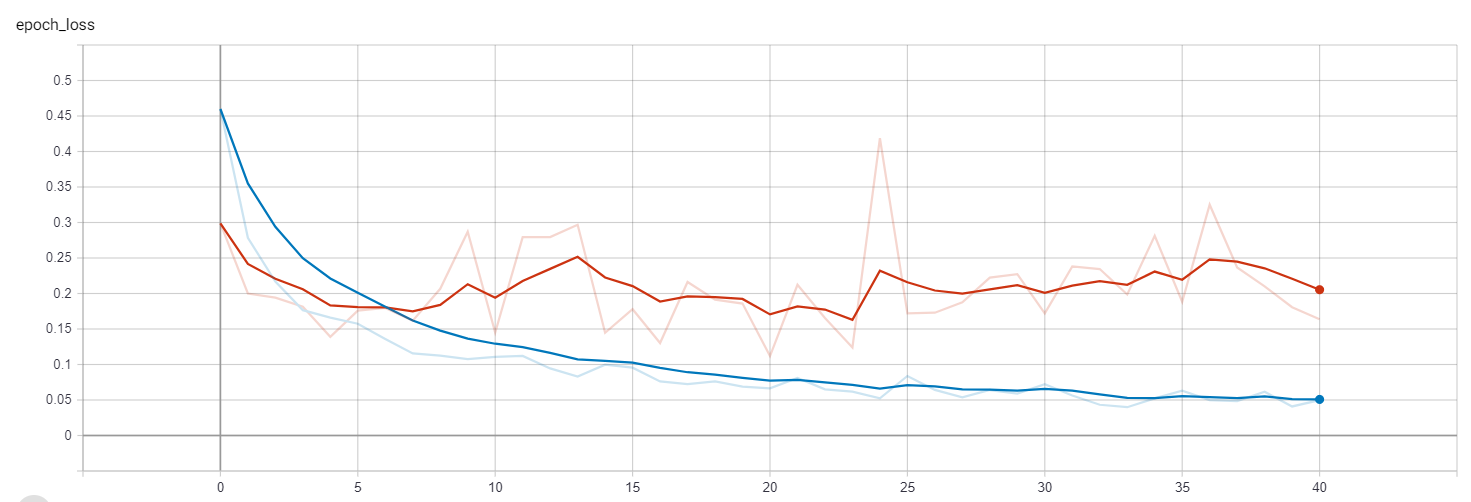
\includegraphics[scale = 0.5, center]{ResNet loss}
	\caption{Loss plot}
\end{figure}
		
		
	
	%end of third chapter
	\chapter{References}
		\section{Links}

\begin{itemize}
	\item GitHub repository of the project: \url{https://github.com/tizianofucci/A2NDLKaggle}
\end{itemize}

\end{document}
